\documentclass[10pt,a4paper]{article}
\usepackage[utf8]{inputenc}
\usepackage{amsmath}
\usepackage{amsfonts}
\usepackage{amssymb}
\usepackage{graphicx}
\usepackage{color}
\usepackage{float}

\usepackage{eurosym}
 
\usepackage{fancyhdr}
 
\pagestyle{fancy}
\fancyhf{}
\rhead{Amsterdam university of applied sciences}
\lhead{Swarming: Research}
\rfoot{Page \thepage}

\definecolor{codegreen}{rgb}{0,0.6,0}
\definecolor{codegray}{rgb}{0.5,0.5,0.5}
\definecolor{codepurple}{rgb}{0.58,0,0.82}
\definecolor{backcolour}{rgb}{0.95,0.95,0.92}
\usepackage{listings}
\lstdefinestyle{cstyle}{
    backgroundcolor=\color{backcolour},   
    commentstyle=\color{codegreen},
    keywordstyle=\color{magenta},
    numberstyle=\tiny\color{codegray},
    stringstyle=\color{codepurple},
    basicstyle=\footnotesize,
    breakatwhitespace=false,         
    breaklines=true,                 
    captionpos=b,                    
    keepspaces=true,                 
    numbers=left,                    
    numbersep=5pt,                  
    showspaces=false,                
    showstringspaces=false,
    showtabs=false,                  
    tabsize=2
}
\graphicspath{ {./images/} }

\begin{document}
\begin{titlepage}
    \centering
    \vfill
    {\Large

    Swarming\\

   
    {\small Research document}\\
        
        \vskip2cm
        {\small M. van Wilgenburg, W. Mukhtar, E. van Splunter, M. Siekerman, T. Zaal and M. Visser}\\
    }    
    \vfill
%    \includegraphics[width=1\textwidth]{WireS4}
    
    \vfill
    \vfill
\end{titlepage}

\newpage

\listoffigures
\newpage

\listoftables
\newpage

\tableofcontents
\newpage


\section{Protocol}
\subsection{Hardware}

For the internal communication between the different systems there are multiple protocols to chose from to transmit data. every subsystem with a microcontroller should be able to communicate with the rest of the system. Because every system should be able to share their information it is necessary to have a multimaster system which allows every system to share their information without being dependent on a single master. To see which protocols are viable multiple protocols will be compared.

Building a modular robot consisting of subsystems, there must be a method to let these "\textit{subsystems}" communicate with each other to exchange relevant information. 

Every subsystem features a micro-controller which must be capable of transmitting and receiving data.  

\subsubsection{TWI}
The name TWI stands for "Two wire interface" which strongly resembles Phillps' protocol $I^(2)C$. Like the name suggests the bus is build up using two wires, one is used for the clock signal and the other is used for the data signal. Each of these wires is connected to the powerline through a pull-up resistor so every subsystem connected to the line can pull the line down which other systems can see. TWI can be used as a multimaster system which means every subsystem can send it's data without being dependend on a single master.

\begin{figure}[H]
        \centering
        \graphicspath{ {./images/} }
        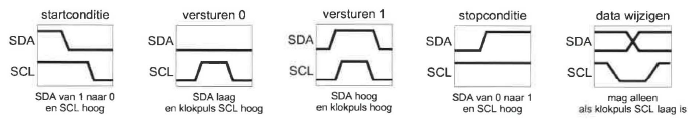
\includegraphics[scale=.6]{datacondities}
        \caption{Data conditions}
        \label{fig:Data conditions}
\end{figure}
In the above figure multiple data and clock combinations are shown, these combinations define the message start, sending a zero, a one and a stopbit. The system that wants to send information starts a message bij changing the datasignal from one to zero on a high clocksignal. All systems that are listening now know one of the systems is going to send a message. Data can be send by changing the dataline from zero to one or the other way around during a low clocksignal, the other systems will read this bit when the clocksignal becomes high again. Once the system is done sending its message it will let the other systems know by sending a stopbit.

\begin{figure}[H]
        \centering
        \graphicspath{ {./images/} }
        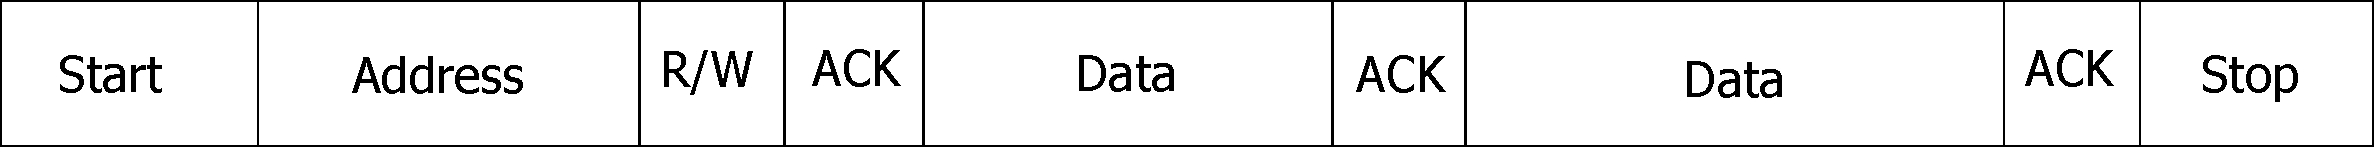
\includegraphics[scale=.6]{TWImessage}
        \caption{Structure of a TWI message}
        \label{fig:TWIstructure}
\end{figure}
In the above picture the structure of a message is shown. As explained before the message starts with a startbit after which a small header follows. The header contains information about who is going to be adressed by the message and if you want to read or write. After this the adressed system will respond with an acknowladge to make sure the information has come across. When the acknowladge is recieved the system will start sending data, followed by and acknowladge from the reciever after every recieved byte of data. when the system is done sending all of its data and recieved the last acknowladge it will send the stopbit which means all communication has ended.
\\
\\
TWI has a few benefits, because it is a simple serial protocol it only uses two wires. this saves a lot of space in the hardware design. Also, it has the possibility to be used as a multimaster system.
The speed of the communication depend on the frequency of the controller that will be used.


\subsubsection{SPI}
SPI or Serial Peripheral Interface is, like it names suggests, a serial interface. This interface can be connected in two ways, each having its own advantage. How this works will be explained using the following figure.
% \begin{figure}[H]
%         \centering
%         \graphicspath{ {./images/} }
%         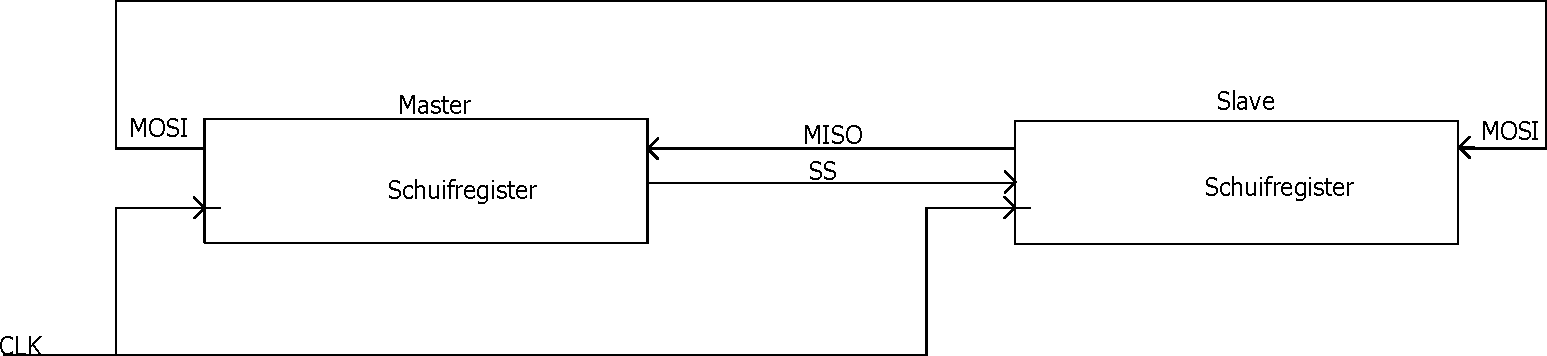
\includegraphics[scale=.6]{SPI}
%         \caption{SPI connections}
%         \label{fig:SPIconnections}
% \end{figure}

\subsubsection{UART}
\subsection{Software}


\newpage
\section{Localization}
Building a swarm of robots, location awareness may be required to ensure an more efficient operation. Implementing location awareness into a swarm of robots could result in better cooperation. For example: exploration based tasks can be executed on a much lower time scale. With location awareness the swarm can spread out evenly making sure that every part of the perimeter will be explored thoroughly. 

With location awareness it is also possible to divide the swarm into multiple groups. Because the location of every individual is available these individual groups can be formed very quickly by selecting the nearest unit. This also enables quick assists when an individual robot gets stuck or needs to execute a task that require more than one unit.

To determine position, not only distance is required, to determine relative position the angle is also required to determine from which angle the units are relative to yourself. However this can result in multiple solutions, the angle could be mirrored.

\begin{figure}[H]
\centering
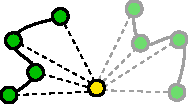
\includegraphics[width=0.9\textwidth]{drolletje.pdf}
\caption{Stationary robot (yellow) cannot compute the relative position of the moving robot (green), since all distance measurements (dashed lines) are invariant to rotations around the stationary robot.\cite{Angle}}
\label{Angle}
\end{figure}

Therefore, in order to leverage the previous trilateration procedure requires coordinating the motion of the robots in a manner that gives every robot a chance to move and ensures that when a robot is moving its neighbors remain stationary. This can also be achieved by the use of stationary anchors.\cite{Angle}

A more efficient solution would be to retrieve the relative orientation opposite to each other. In combination with the relative distance every robot knows the exact relative position of all the other robots in range of the network.
\newpage

\subsection{Relative Distance}
Relative distance can be measured using various methods. The most common methods are \textit{"Received Signal Strength Indication"} and \textit{"Time Of Flight"} abbreviated as RSSI and TOF. 

\subsubsection{Received Signal Strength}
A method to determine distance can be implemented using Received Signal Strength abbreviated as "RSSI". Typically RSSI is a measure of dBm, which is ten times the logarithm of the ratio of the power (P)
at the receiving end and the reference power (Pref). Power at the receiving end is inversely proportional to the
square of distance.\cite{RSSI} Hence RSSI could potentially be used as an indicator of the distance
at which the sending unit (robot) is located from the receiving unit.\cite{RSSI}

RSSI is defined as ten times the logarithm of the ratio of power of the received signal
and a reference power (for example 1mW). It is known that power dissipates from its source
as it moves further out. As mentioned earlier the relationship between power and distance is that power is inversely
proportional to the square of the distance travelled. \cite{RSSI}

In theory it seems as a suitable implementation for the purpose, determining relative distance between
different units. However various test results have shown that RSSI is only reliable under certain circumstances.
Test results have shown that if the orientation of the sending or receiving unit changes it becomes very unreliable.
The graphs below show the reliability of RSSI when the direction is being altered.\cite{RSSI}

\begin{figure}[H]
\centering
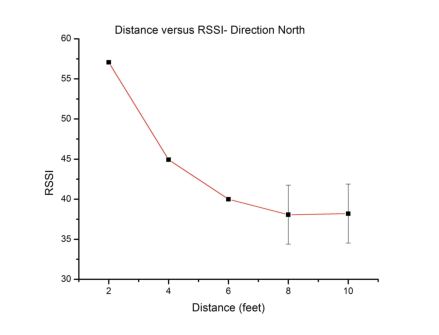
\includegraphics[width=0.9\textwidth]{North.pdf}
\caption{Distance versus RSSI plot showing inverse non linear
relationship.\cite{RSSI}}
\label{North}
\end{figure}

\begin{figure}[H]
\centering
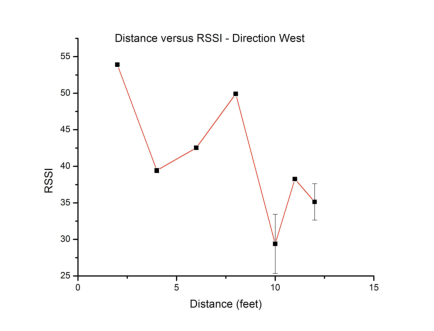
\includegraphics[width=0.9\textwidth]{West.pdf}
\caption{Distance versus RSSI plot showing lack of
reliability when tested in a different direction.\cite{RSSI}} 
\label{West}
\end{figure}

\begin{figure}[H]
\centering
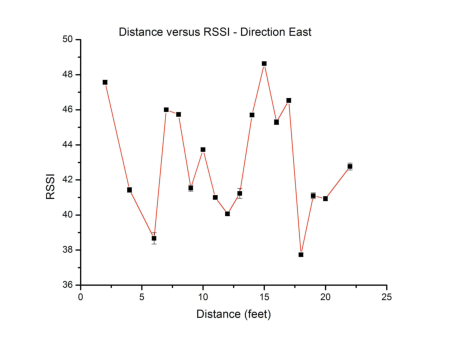
\includegraphics[width=0.9\textwidth]{East.pdf}
\caption{Distance versus RSSI plot showing lack of
reliability when tested in a different direction.\cite{RSSI}} 
\label{East}
\end{figure}
\newpage


Even though RSSI was very promising in many studies, through multi directional experiments it became clear that even under ideal conditions with weather and interference controlled, the RSSI data could not be relied upon. At times the data was correct showing the expected inverse square relation with distance and at other times it didn't.\cite{RSSI}


\subsubsection{Time Of Flight}
Another common method to determine relative distance is Time Of Flight abbreviated as "TOF". Time Of Flight describes a method that measures the time that an particular wave takes to travel a distance trough a medium. The wave can be acoustic, electromagnetic and light.

For relative distance measurements Time Of Flight is often combined with Time Difference Over Arrival abbreviated as "TDOA". Combining these methods enables relative distance measurements to specific units/nodes. TDOA measures the time difference between the transmission and arrival of a wave. With the velocity of propagation times the travelled time de relative distance between two or more nodes can be determined. However TOF also features certain limitations being clock synchronization, noise, sampling and multipath channel effects.\cite{TOF} 

\textit{Clock Synchronization}
TOF ranging systems need to estimate the time of transmission and arrival and comparing this with a common time reference.\cite{TOF} If the different time references are not perfectly synchronized a time offset error occurs. With the faster the propagation speed, the greater the error in distance. 

\textit{Sampling}
Using Light or electromagnetic waves to determine the relative distance can add several limitation. Due to the high velocity propagation (being nearly equal to equal of the velocity propagation of light) sampling this signal requires very high clock rates to do so. It would take a 15GHz clock to achieve one centimetre resolution.\cite{Arduino}

in the 1960's, Tektronix invented a sampling method with a oscilloscope that could measure signals in the GHz range without using high speed clocks. This method is called Sequential Equivalent Time Sampling abbreviated as "SETS". The SETS acquires one sample per trigger see figure \ref{SETS}. When a trigger is detected a sample is taken after a very short, but well defined delay. When the next trigger occurs a small time increment "Delta T" is added to this delay and the digitizer takes another sample. This process is repeated many times with "Delta T" added to each previous acquisition, until the time windows is filled.\cite{SETS} In figure \ref{SETS2} another example of an sinusoidal signal is displayed using the SETS method. 

Using the SETS method enables the use of waveform with an velocity propagation nearly equal to equal to the speed of light. However implementing a advanced SETS circuit is required to reach accuracy of less than 1 meter indoors.\cite{TOF} However using waveforms with a high velocity propagation enables faster data transfers and a larger range.\cite{TOF}

\begin{figure}[H]
\centering
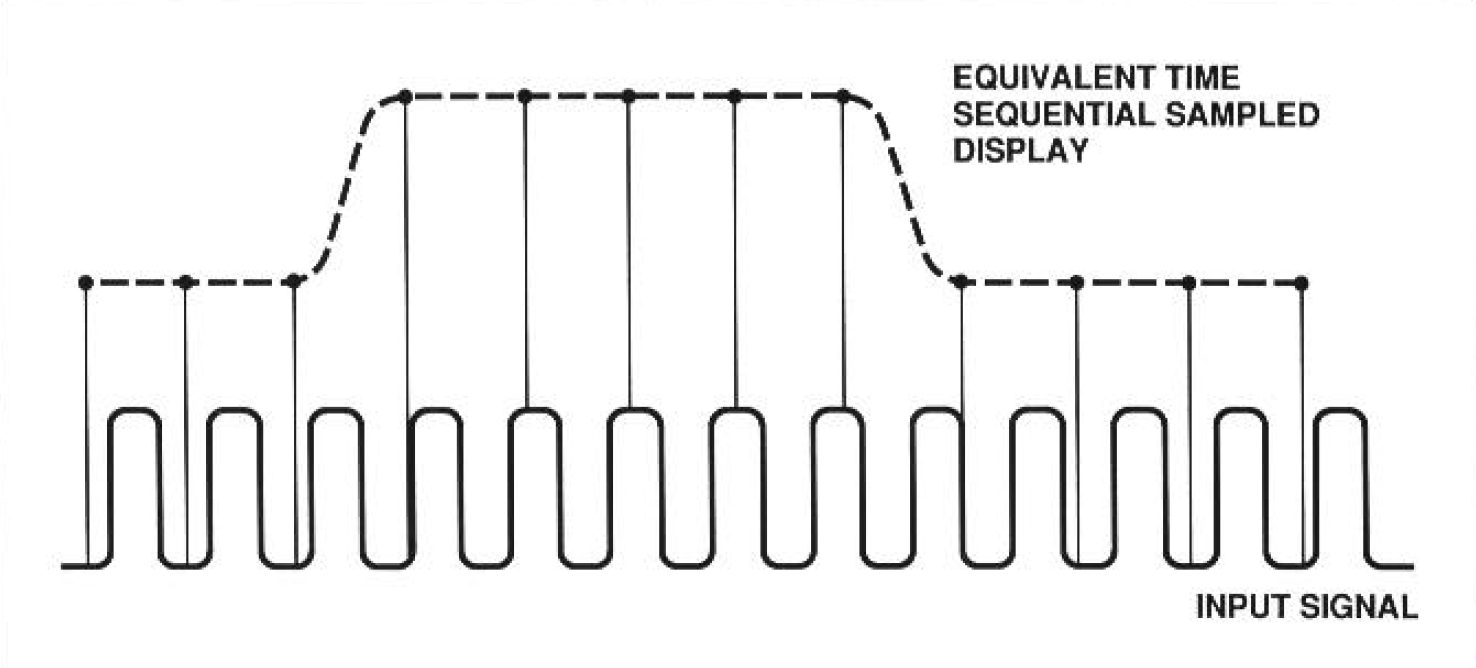
\includegraphics[width=0.9\textwidth]{SETS.png}
\caption{In sequential equivalent time sampling a singel sample is taken for each recognized trigger after a delay which is incremented after each cycle.\cite{SETS}} 
\label{SETS}
\end{figure}

\begin{figure}[H]
\centering
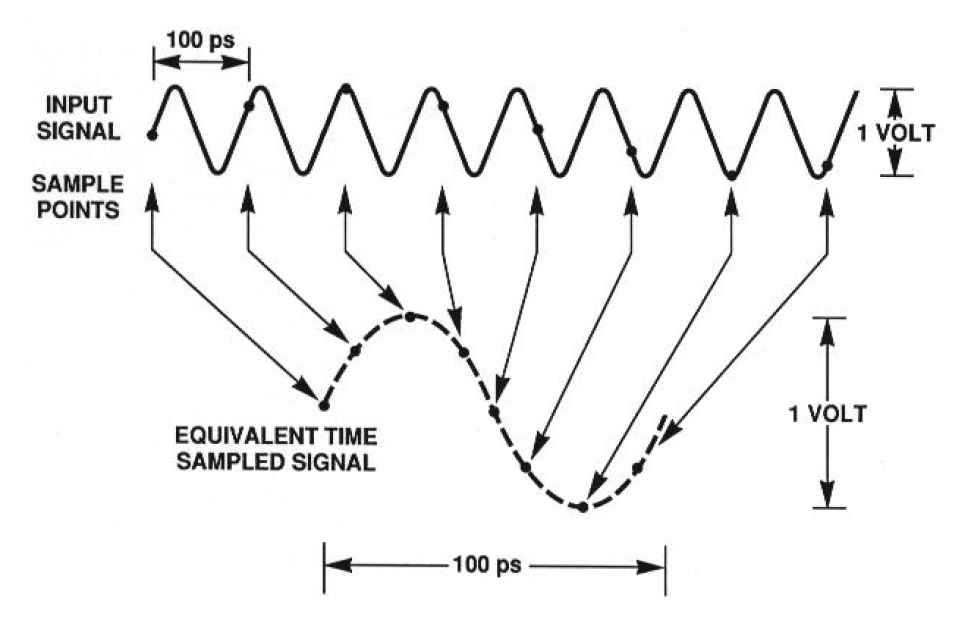
\includegraphics[width=0.9\textwidth]{SETS2.png}
\caption{Example equivalent time sampled signal.\cite{SETS}} 
\label{SETS2}
\end{figure}
\newpage

\subsection{Conclusion}
Different studies have shown that Received Signal Strength can theoretically measure distance accurately. However RSSI seems to be very unreliable in many circumstances which leads to not being viable for distance measurements with moving robots. 

Time Of Flight has been very promising, however using electromagnetic signals (For example RF, WI-FI or Bluetooth) the acceptable accuracy starts at from a minimum range of 1-2 meters which leads to unreliable to no useful information at all in the range of 1-2 meters. This minimum range could be narrowed using an Sequential Equivalent Time Sampling Circuit, however such a circuit is complex to develop. However using waveforms with a lower velocity propagation can lead to accurate close range measurements. In this case Time Of Flight suits better for the required use, being more accurate and reliable see figure \ref{RSSIvsTOF}.\cite{TOF}

\begin{figure}[H]
\centering
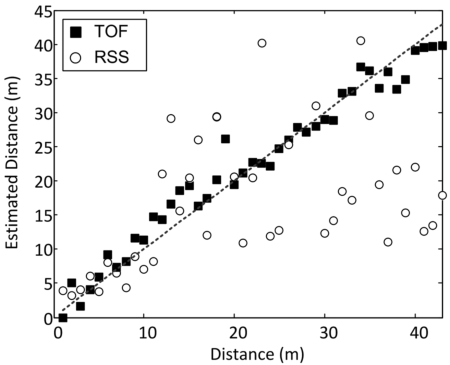
\includegraphics[width=0.9\textwidth]{RSSIvsTOF.pdf}
\caption{Accuracy RSSI vs TOF.\cite{TOF}} 
\label{RSSIvsTOF}
\end{figure}

Determining relative distance does not lead to localization to do so a angle is required. 
\newpage

\section{Onderzoek}
Hier tekst plaatsen

\subsection{Propulsion,Actuators and Effectors}

In this chapter the sub-questions about the propulsion, actuators and effectors are researched and answered. First of all, the possible types of propulsion will be researched. Then the various kinds of actuators with a suitable effector will be considered. Depending on the situation different types of propulsion is used. For example a robot that operates in an environment with water would not be implemented with DC motor drivers and tyres. The robot build in this research should be able to operate on Mars in the future. Therefore the robot cant get stuck easily since that will cost millions, since the robot cannot complete his mission. Since swarming and not propulsion is the main goal of this research a simple way of locomotion would suffice. However there should be the possibility to implement a different kind of propulsion in the future, so that the robot can be used on Mars. 


%In dit hoofdstuk worden de deelvragen over de aandrijving, actuatoren en effectoren beantwoord. Allereerst zal er onderzocht worden welke soorten aandrijving er mogelijk zijn.Vervolgens zal er worden gekeken welke actuatoren er gebruikt kunnen worden en hoe de energie van de actuator gebruikt kan worden om de robot voort te bewegen. Als laatste wordt er gekeken welke effectoren nodig zijn. Robots worden op veel verschillende manier aangedreven, afhankelijk van de situatie.Bijvoorbeeld een robot die op het water moet opereren zal niet vaak met DC motoren met wielen worden ge\"implementeerd. In dit onderzoek kijken we naar een robot die in de toekomst mogelijk naar mars gestuurd kan worden. Dan kan de robot niet zomaar vast komen te zitten, aangezien er dan miljoenen voor niks verloren gaan. Omdat er eerst met een vereenvoudigde werkelijkheid wordt gewerkt is het vooral belangrijk dat de robot eenvoudig kan voortbewegen. Wel moet er ruimte zijn om later een andere module te kunnen aansluiten zodat hij ook op mars zich zou kunnen voortbewegen. 

\subsubsection{Effectors}
The way a robot moves is determined by its effector with his corresponding actuator. Possible types of effectors are:

%Door een effector aan een actuator de koppelen kan een robot zich voortbewegen. Mogelijke effectoren kunnen zijn:

\begin{itemize}
\item Wheels
\item Leg(s)
\item Catepillar tracks
\item Air cushion  
\item Propeller 
\item (Superconductor)
\end{itemize}

Each of these effectors have pro's and con's in different situations. Tyres are easily implemented, but there are various ways to implement these. The amount of tyres used will affect the handling of the robot. With a minimum two tyres, movement can already be realized. The downside is that driving with two wheels is not stable, only with algorithms that can balance the robot stable movement can be accomplished. It would be easier to implement more than two wheels so that the robot is more stable and movement is easier. 


  
%hier gebleven met vertalen
Elke van deze effectoren hebben voor en nadelen in verschillende situaties.\\Wielen zijn eenvoudig te implementeren, er kunnen verschillende aantallen wielen worden aangebracht. Het aantal wielen heeft wel invloed op het rijgedrag van de robot. Met twee wielen kan er worden gereden, mits de robot in balans wordt gehouden. Dit kan worden gedaan door middel van een zwenkwiel, of door een regelsysteem te bedenken dat de twee wielen de robot in balans houden. Dit laatste kost veel energie en is niet eenvoudig. Met drie wielen staat de robot al een stuk stabieler. Het nadeel hiervan is dat sturen soms moeizaam kan zijn. Met vier wielen is de robot nog stabieler en kan er op verschillende manieren worden gestuurd. De wielen kunnen tegengesteld worden aangedreven waardoor de robot draait. Dit kost wel meer energie dan nodig is aangezien er extra wrijving ontstaat. Een optie is de voorste wielen te laten draaien, waardoor de robot in de richting van de wielen zal voortbewegen. Zoals bij een auto het geval is. Dit is weer lastiger te implementeren aangezien er een soort van stuurmechanisme moet worden bedacht. 

\subsubsection{Actuatoren}

De keuze van de actuator hangt sterk samen met de effectoren.

\subsubsection{Aandrijving}

\newpage
\subsection{Swarm communication}
There are several requirements to realise a robot swarm. Each member of the population needs to communicate with the rest of the swarm. To give the members full freedom of movement it is also usefull to make the communication wireless. It is important that the population size of the swarm is dynamic, because of the scalability of the swarm. As mentioned earlier a swarm does not have a master. So each member needs to be capable to maintain the network. These networks also must be able to reroute around nodes that have been lost. \cite{Swarmwiki}\cite{swarmintelligence}

The following subsections are 
\begin{itemize}
\setlength\itemsep{0em}
    \item Network topology
    \item Network realibility and robustness
    \item Routing protocol
    \item Data distribution
    \item Wireless mesh network
    \item Wireless network implementations
    \item Conclusion
\end{itemize}



\subsubsection{Network topology}
Several topologies exist to form a network. Figure \ref{fig:STAR}, \ref{fig:RING}, \ref{fig:BUS} and \ref{fig:WMN} illustrate four network topologies as an example. Each topology has it's own benefits and cons which are discussed in this section.

\begin{figure}[H]
\minipage{0.32\textwidth}
  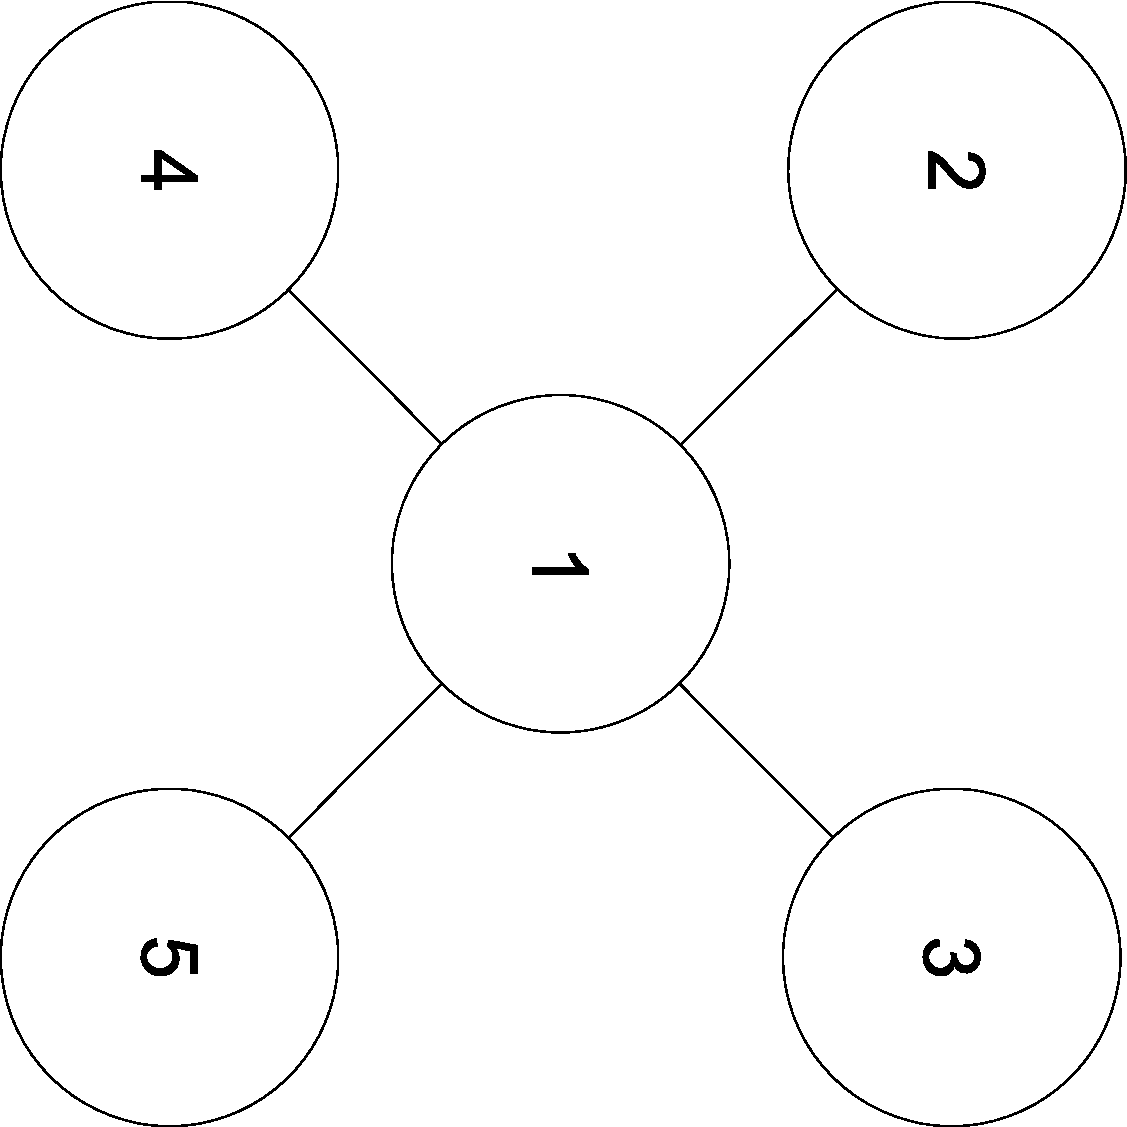
\includegraphics[angle=90,width=\linewidth]{STAR}
  \caption{A star network topology, devices are connected to a central device (in this case device 1.)}\label{fig:STAR}
\endminipage\hfill
\minipage{0.32\textwidth}
  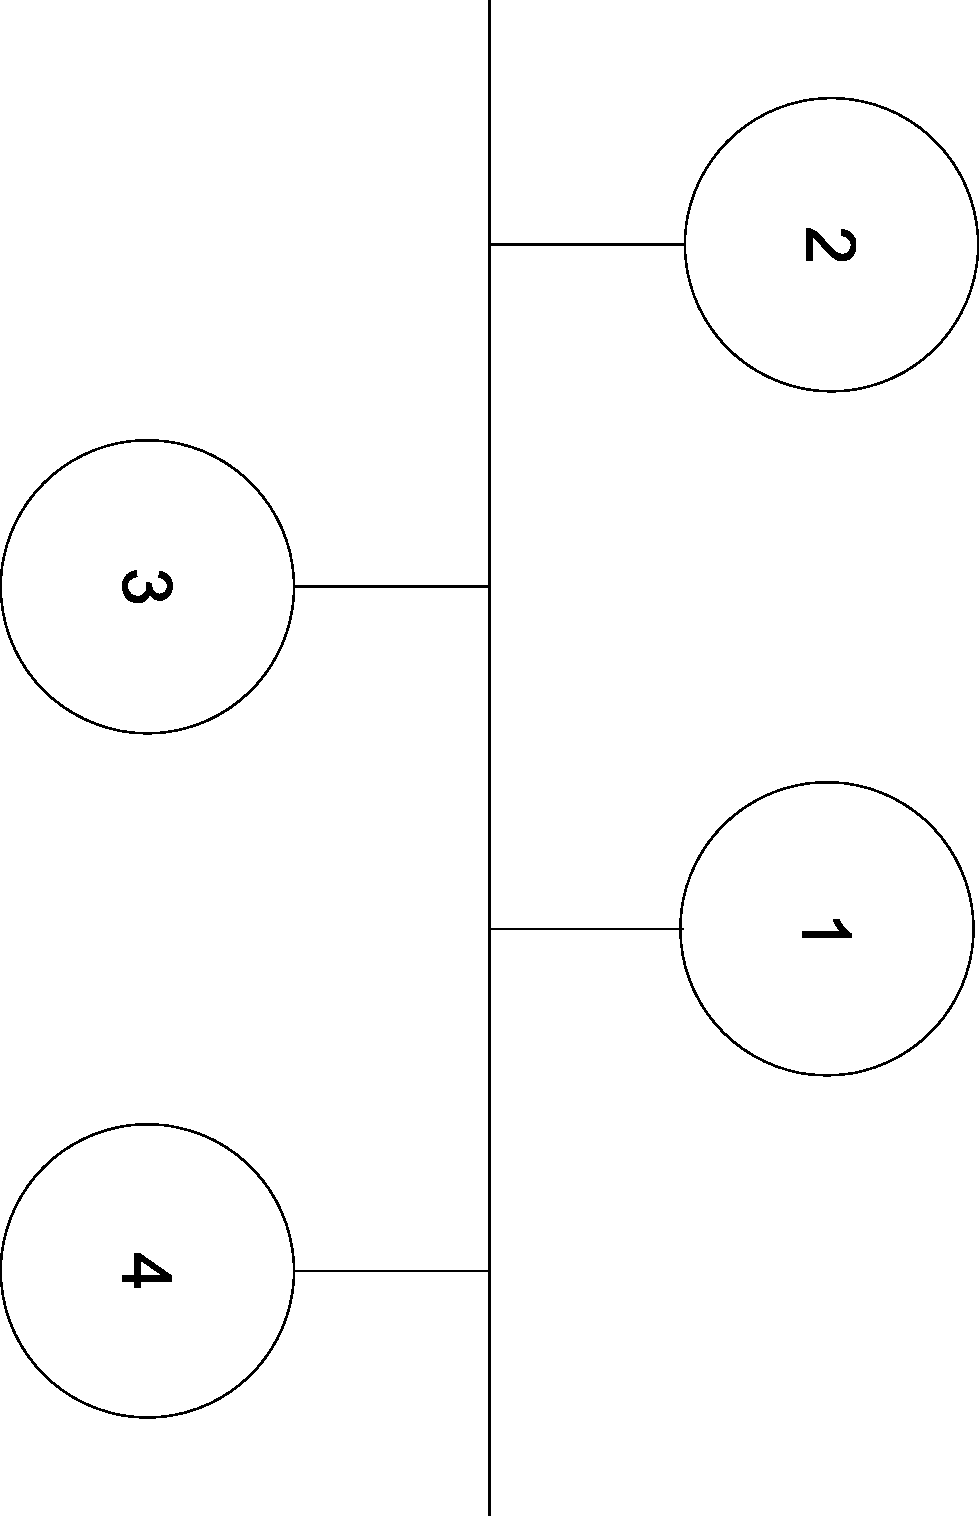
\includegraphics[angle=90,width=\linewidth]{BUS}
  \caption{A bus topology, every device is on a common link.}\label{fig:BUS}
\endminipage\hfill
\minipage{0.32\textwidth}%
  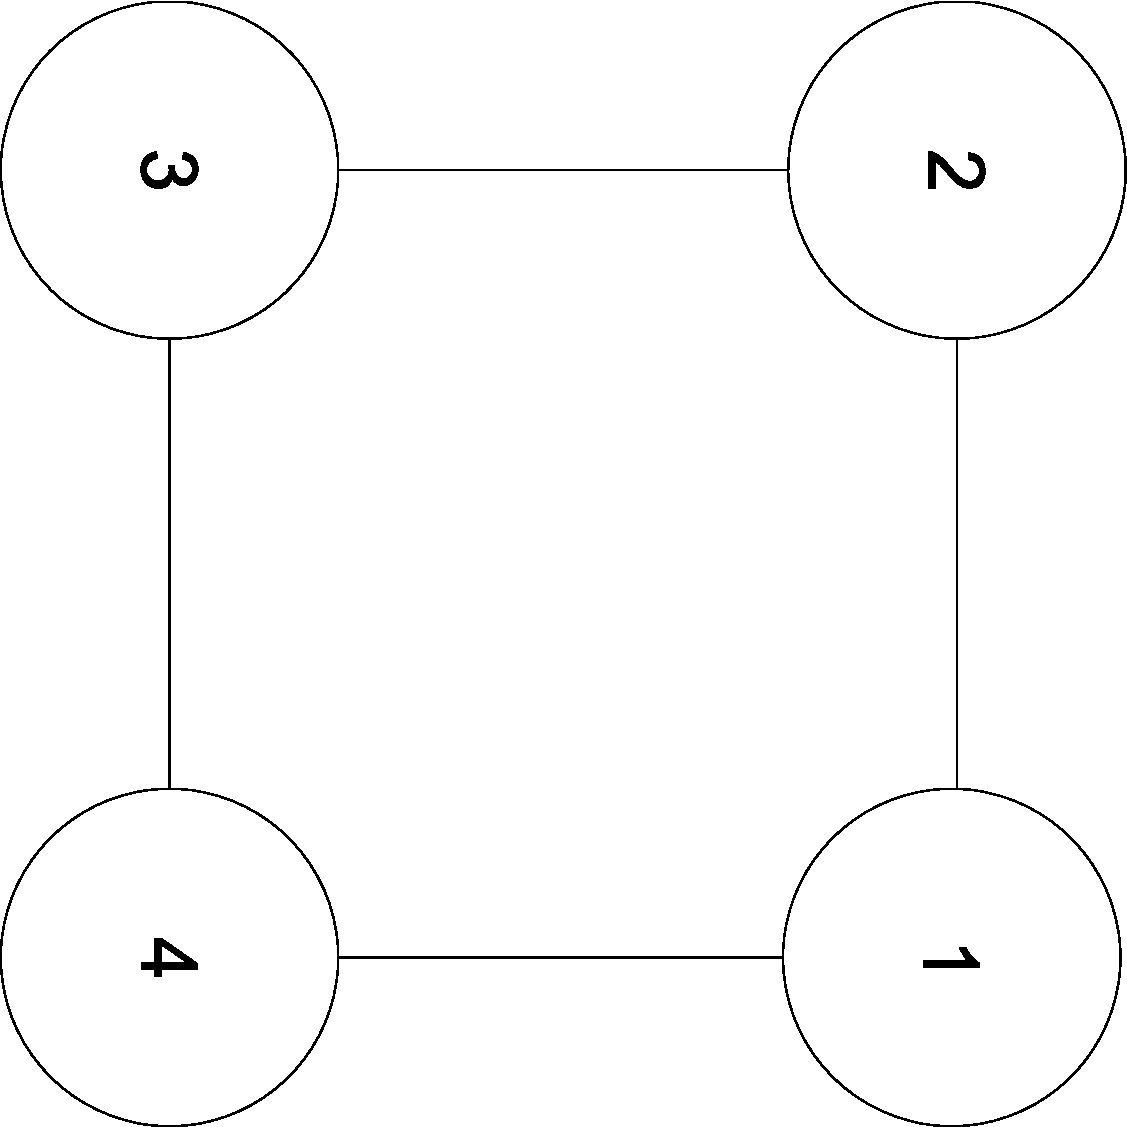
\includegraphics[angle=90,width=\linewidth]{RING}
  \caption{A ring topology, each device is connected to the next nearest device.}\label{fig:RING}
\endminipage
\end{figure}

\textbf{Star network}\\
The star network in figure \ref{fig:STAR} uses the device marked as '1' as an central switch to reach out to other devices.\cite{starwiki} When the central device fails the network will stop working. This means that the star topology is not suitable as a swarm network.


\textbf{Ring network}\\
Devices in a ring network ar always connected to two other devices as displayed in figure \ref{fig:RING}. This means that there are atleast three devices in a ring network. The data distributions is unidirectional, with the traffic travelling clockwise or anticlockwise around the ring. \cite{ringwiki} This topology has it's limitations when one or more devices become isolated due to a device faillure or cable break. This problem can be solved by using a dual ring, which makes the network redundant. Because of the network topology, in which n nodes are connected serially, the communication delay is proportional to the number n devices in the network. The bandwidth is also shared between all the devices. \cite{ringwiki} It is possible to create a swarm network with a ring network but it is far from ideal.

\textbf{Bus network}\\
In a bus network the devices are connected to a linear half-duplex link. \cite{bustopology} A bus network has the advantage that it is easy to connect devices to and it works well in small networks. A disadvantage when using a bus for swarming is that the entire network shutsdown when there is a break in the main connection. 
This makes the network not dynamic.

\textbf{Mesh network}\\
To create an network with the characteristics described in the previous section a (wireless) mesh network ((W)MN) is a possible solution. A mesh network relies on communication nodes in which data is distributed. Such a network uses multi-hopping to transport data.\cite{multi-hopwirelessnetworks} All of the communication nodes cooperate in the distribution of data in the network. Each node of the network is connected to one or more nearby in range node(s) and forwards data on behalf of the other nodes. \cite{meshnetworking} An example of a mesh network is illustrated in figure \ref{fig:WMN}. It is possible but not necessary to connect one or more clients of a mesh network to the internet. Thus the client connected to the internet functions as a gateway for the other clients in the network. \cite{wirelessmeshnetworksopportunitiesandchallenges}

\begin{figure}[H]
   \centering
   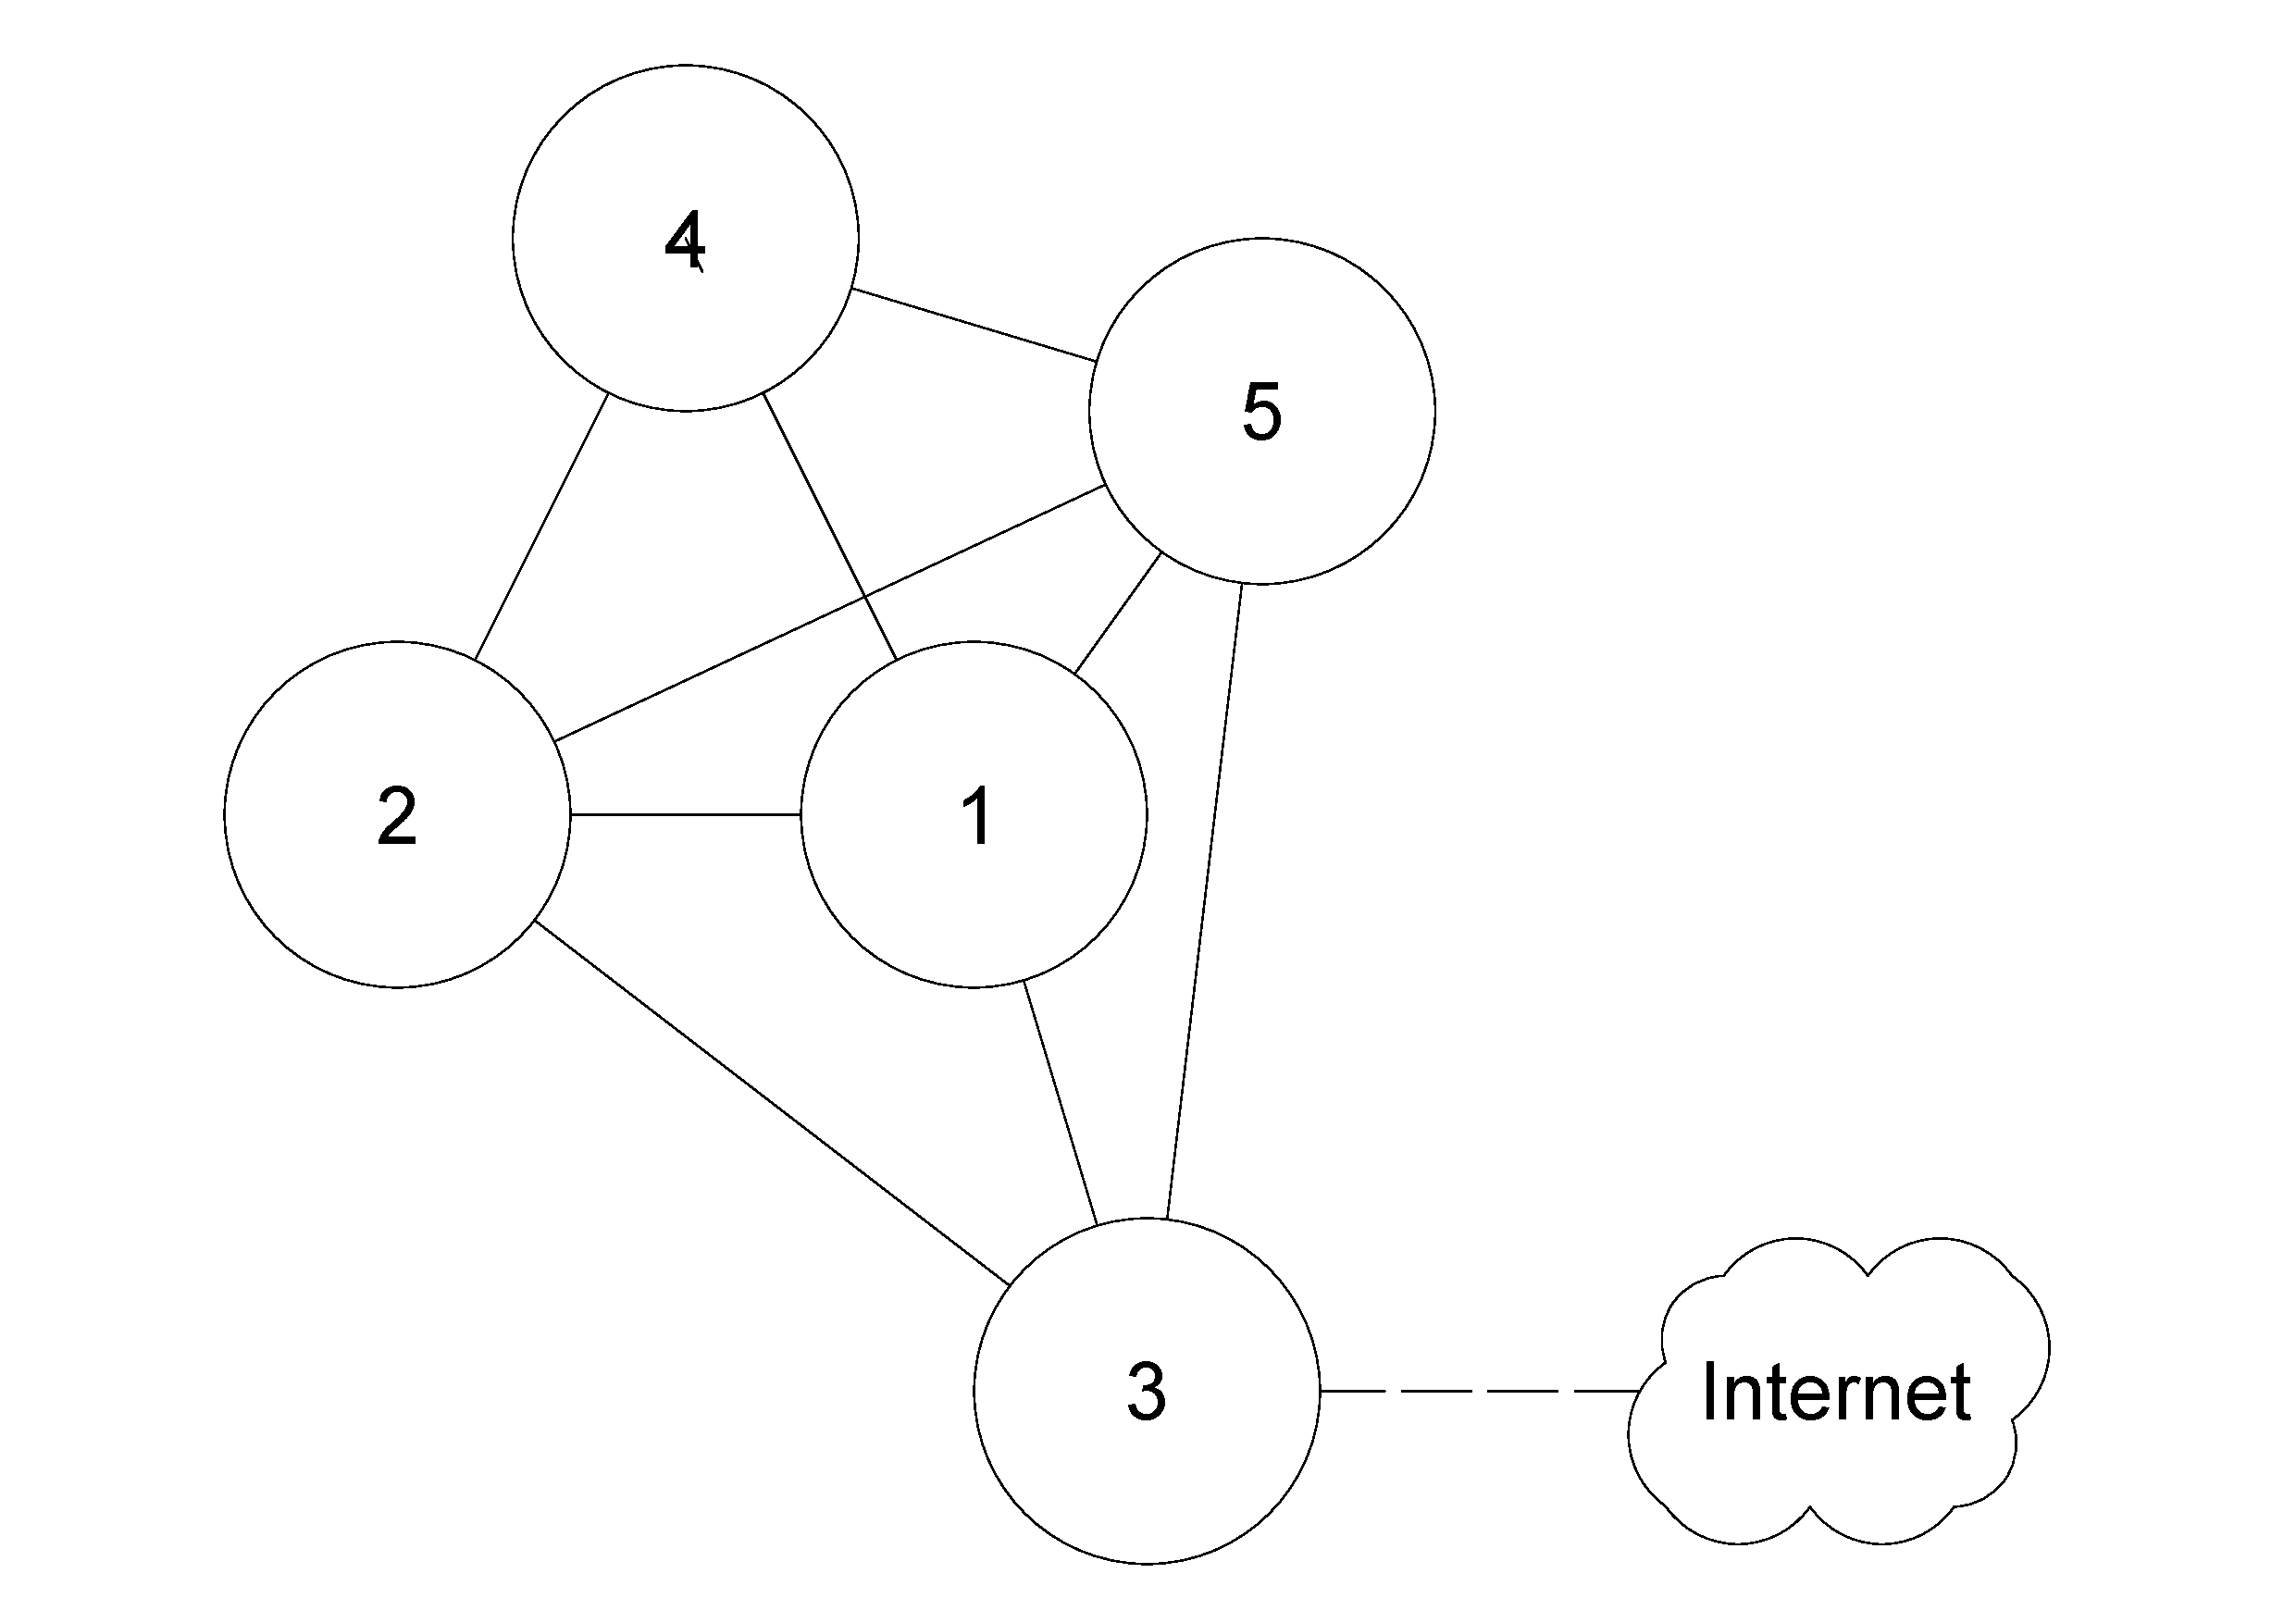
\includegraphics[width=1\textwidth]{WMN}
   \caption{An example of a wireless mesh network with 5 clients and an optional internet connection. The connections made in this example are random.}
   \label{fig:WMN}
\end{figure}

\textbf{Comparison and conclusion}\\
When the network topology's are compared with each other, the mesh network satisfies the desired requirements. Although it is harder to implement due to mutual connections, it has the best data coverage. In this situation, a mesh network would be the best choice.

\subsubsection{Network realibility}
To ensure a realiable network, self-organization and topology control algorithms are needed.\cite{WMN1} Possibly important and usefull (wireless) network characteristics are \cite{position-based}:
\begin{itemize}
\setlength\itemsep{0em}
    \item Low construction costs
    \item Energy efficient (power aware)
    \item Cost aware
    \item Robust - Able to withstand a lost or broken client or connection
    \item Guaranteed delivery
\end{itemize}

Mesh networks can use self-healing algorithms such as Shortest Path Bridging (SPB) to restore and reroute the connection around broken nodes/clients. Shortest path bridging calculates the most favorable connections to the clients with the lowest path costs. \cite{SPB} Other usefull algorithms such as shortest path, greedy, shortest cost path, cost aware, power aware, are listed in \cite{position-based} with their characteristics. In this research only the most suitable algorithms will be discussed. 

The distance between neighboring nodes can be estimated on the basis of signal strengths or time delays in direct communications. The exact positions can for example be estimated by using positioning systems such as GPS (Gereral positioning system). \cite{locationsystemsforubiquitouscomputing} 




The shortest path route protocol uses information such as the hopcount and distance between clients to calculate the shortest route. Hopcount stands for the amount of clients that are passed by. The shortest cost path route protocol also takes account for the energy required for each routing task. The goal of this protocol is to minimize the total energy cost. According to \cite{position-based} it is not desireable or if possible to avoid to memorize routes or past traffic in mobile ad hoc networks. This is because of the mobility of clients in the network and constantly changing infrastructure.


The scalibility of each algorithm means the posibility to adjust the scale of the network by adding or removing clients to the network. According to the research done in \cite{geographicalrouting}\cite{scalablelocation} routing algorithms without geographic locating (precize localisation) are not scalable and won't work well in large networks. 

A realiable network has a routing algorithm/protocol that includes distributed operating, loop freedom, demand-based operation and sleep period operation. Loop freedom means that the protocol is able to detect loops in the network and eliminates those. For example, data could be floating around in the network. Sleep period operating means that the clients that are not needed go into a 'sleep mode' when it's temporarily inactive.\cite{position-based}


\subsubsection{Data distribution}
There are several strategys to distribute a package of data in a network. The following enumeration show three strategy's:
\begin{itemize}
\setlength\itemsep{0em}
    \item single-path
    \item multipath
    \item flooding
\end{itemize}

The single-path strategy is an example of the shortest path route protocol. In the single-path strategy only one packet of data in distributed in the network at a time. Which is desireable for the network capacity which is barely affected. Although the capacity is not affected, it is possible that a package is received later, because of an missing or inactive node in the path. \cite{position-based}

The other strategy, multipath, sends out multiple packets of data trough recognizable paths. Flooding strategy litterly floods the network with data packages. In case of wireless networks, the single-path strategy is preferred because of the power and bandwidth limitations in wireless networks. \cite{position-based}



In figure \ref{fig:greedyrouting} a greedy routing scheme is displayed. The node S contains the data package and D is the destination of the package. 

\begin{figure}[H]
   \centering
   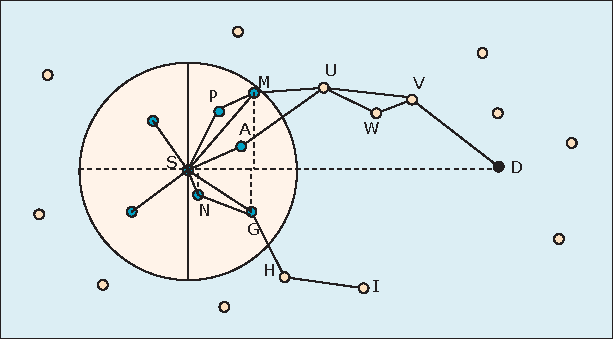
\includegraphics[width=1\textwidth]{greedyrouting}
   \caption{Greedy round scheme found in \cite{position-based}. "S selects M in MFR path SMUVD, G in greedy path SGHI that
fails to deliver, A in direction-based-path SAUWVD, P in power path
SPMUWVD, N in NFP/NC path SNGHI that fails to deliver."}
   \label{fig:greedyrouting}
\end{figure}

The principle of greedy routing is that it is trying to get closer to the destination based on local information. Thus the data package is forwarded to the client/node which is the most suitable from a local point of view. \cite{geographicrouting} "Greedy schemes have a performance close to performance of optimal shortest path (weighted) algorithm for dense graphs, but have low delivery rates for sparse graphs. Schemes that guarantee delivery may have high communication overhead for sparse graphs." \cite{position-based} The most efficient algorithm for path bridging depends on the situation where the clients are operating in which is described in \cite{position-based}.


\subsubsection{Wireless mesh network}
A mesh network (MN) is a dynamically self-organized and configured network. \cite{WMN1} As described earlier the swarm network is dynamic in size and mutual distance. Because of the size and mobility of the swarm it is not practical to use wired connections between de members of the swarm. So a wireless mesh network (WMN) is needed. Therefore a wireless connection between the members is necessary.

Despite the practical benefits of wireless networks, today's wireless networks still cannot offer the same level of sustained bandwith as their wired brethren. The bandwidth is for instance affected by interference from adjacent hops on the same and neighboring paths. \cite{architectureandalgorithmsmultichannelwirelessmeshnetwork} One of the most important drawbacks is that each client needs to be in transmitting and receiving range to atleast one of the other clients to be connected to the network. \cite{wirelessmeshnetworksopportunitiesandchallenges} Another con is that the data rate falls quickly when increasing the distance between transmitter and receiver, which doesn't or barely apply to wired networks. \cite{architectureandalgorithmsmultichannelwirelessmeshnetwork} The complexity of an WMN network is also a main drawback. It is relatively easy to design a WMN, but it is difficult to achieve an optimum performance while ensuring security and robustness.\cite{wirelessmeshnetworksopportunitiesandchallenges} 

Each node or client in the network is able to create an ad hoc network to maintain the mesh connectivity, this is called "client WMN's". These networks are able to reroute around nodes that have been lost. On large scale projects wireless mesh networks are costefficient because of the saving of wired connections.\cite{meshnetworking} 

Nevertheless, the client mobility weigh out the cons described earlier. So solutions must be found to overcome these drawbacks


\subsubsection{Meshed architecture}


Methods to adress meshed networks are:
\begin{itemize}
\setlength\itemsep{0em}
    \item Adaptive robust tree (ART)
    \item Meshed adaptive robust tree (MART)
\end{itemize}

\textbf{Adaptive robust tree (ART)}\\
Adaptive robust tree is a meshed tree routing approach to address the nodes. Each node is adaptively addressed during the tree formation. It is desireable that the tree is free of single point failures (SPOF). This means that there is always a redundant path if a node fails, but that's not always possible in non-mesh networks. Each node keeps track of an ART table (ARTT), to map it's branches. In this table the adresses of the connected branches are stored.

ART knows three phases; the initialization, operation and recovery phase. In the initialization phase the tree is formed. The tree formation starts at the root and grows by adding nodes to the tree. The nodes get an adress assigned, when all nodes are joined. Thereafter, the number of nodes are counted in the tree as shown in figure \ref{fig:treenumbers}.

\begin{figure}[H]
   \centering
   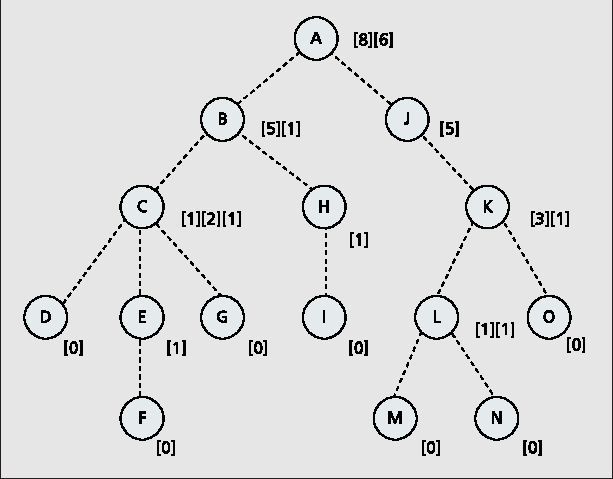
\includegraphics[width=1\textwidth]{treenumbers}
   \caption{An example of a wireless mesh network with 5 clients and an optional internet connection. The connections made in this example are random.}
   \label{fig:treenumbers}
\end{figure}

The following phase is the operation phase, where small amount of nodes are still able to join, but when the change becomes to big, the network goes in to initialization mode again. When a part of the tree becomes broken, the recovery phase becomes active for the affected part.

\textbf{Meshed adaptive robust tree}\\
With an ART tree it is possible to create a MART (Meshed adaptive robust tree). Figure \ref{fig:meshtree} illustrates a MART, in this figure there are already connections added that make a mesh network. From the point of view from every node in the network, there still is a tree form. In this mesh network, each node has a redundant path if a connection is broken, so it is SPOF free.

\begin{figure}[H]
   \centering
   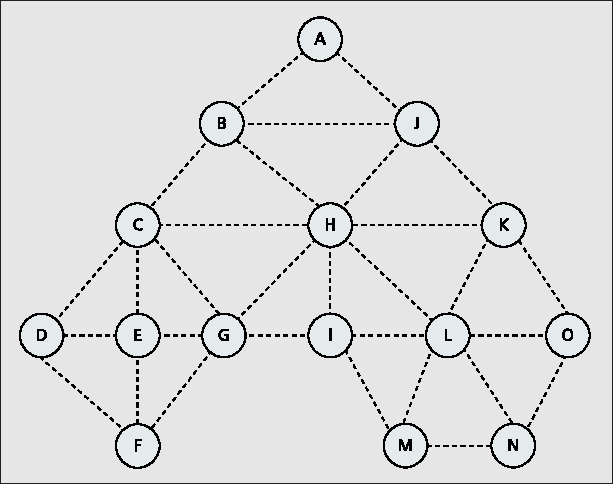
\includegraphics[width=1\textwidth]{meshtree}
   \caption{Meshed ART formation, from \cite{emergingstandarsforwirelessmeshtechnology}}
   \label{fig:meshtree}
\end{figure}

With a MART, it is possibile to reroute a connection to reduce the path cost in comparison with ART. Most of the time, the transission from ART to MART, removes some SPOFs.

\textbf{Mesh wireless personal area networks}\\
A mesh wireless personal area networks



\subsubsection{Wireless network protocols}



Standards for wireless mesh networks:\cite{emergingstandarsforwirelessmeshtechnology}

\begin{table}[H]
\centering
\caption{Types of mesh networks and related marketing alliances \cite{emergingstandarsforwirelessmeshtechnology}.}
\label{meshstandard}
\begin{tabular}{|l|l|}
    \hline
    \textbf{Name}         & \textbf{Corresponding standard} \\ \hline
    WMAN mesh (WiMAX)     & IEEE 802.16a                    \\ \hline
    WLAN mesh (WiFi)      & IEEE 802.11s                    \\ \hline
    LR-WPAN mesh (ZigBee) & IEEE 802.15.5                   \\ \hline
\end{tabular}
\end{table}



There exist several techniques to accomplish this method 
Examples of possible protocols:
The following wireless protocols are defined as short-range (a range of 10-100m) communication protocols:
\begin{itemize}
\setlength\itemsep{0em}
    \item IEEE 802.11 a/b/g/ac (WiFi) \cite{IEEE80211timeline}
    \item IEEE 802.15.1 (Bluetooth)
    \item IEEE 802.15.4 (ZigBee)
    \item IEEE 802.15.3 (Ultra-wideband)
    \item SwarmBee
\end{itemize}

\textbf{IEEE 802.15.1 Bluetooth}\\
Bluetooth is designed for short-range communication which uses wireless radio systems. The main purpose of Bluetooth is to create a wireless connection between computer peripherals such as; keyboards and mice. These applications are also known as wireless personal area networks (WPAN). \cite{comparitivestudywirelessprotocols} Bluetooth is an ad hoc network, which means that the network is formed spontaneously.\cite{tcipbook}

Bluetooth uses the industrial scientific and medical (or short: ISM) band for receiving en transmission data. The ISM band ranges from 2,400 to 2,4835 GHz in the Netherlands. \cite{frequencyandsnetherlands} Frequency hopping spread spectrum (FHSS) is used to spread out the power over the full bandwidth. After the transmission of each packet, Bluetooth will hop/change to another channel. The ISM band consists of 79 channels with 1MHz each. Changingin frequencies also helps to avoid collision with other networks. But it is still possible that a collision takes place. When a collision happens, the data is resend on another channel untill the transmittion is succesfull.

\begin{figure}[H]
   \centering
   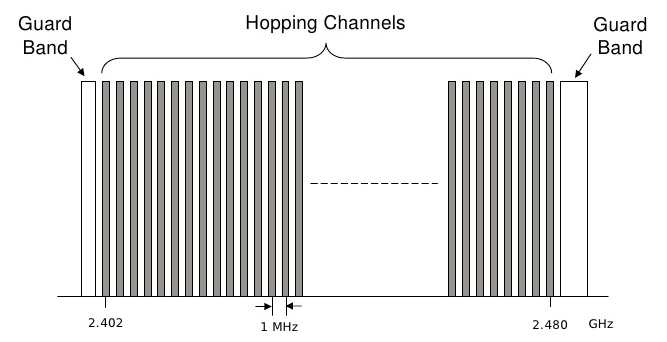
\includegraphics[width=1\textwidth]{bluetoothfh}
   \caption{Bluetooth frequency hopping spread spectrum (FHSS) from \cite{bluetoothspectrum}}
   \label{fig:bluetoothfh}
\end{figure}

Bluetooth consists of two network topologies: a piconet and scatternet. The piconet has one or more slaves serving one master \cite{bluetoothpiconet}. In a piconet the master synchronizes the master's clock and shares his bluetooth device adress at the first connection. The data packet is called a frequency-hopsynchronization packet (FHS packet). The data send in the FHS packet is used to calculate the sequence of frequency hops that all devices in the piconet will follow. Each client in the networks tracks the native- and masters clock, so it will know on which frequency the client needs to transmit or receive.

Each piconet has one master which has an unique Bluetooth device adress and clock. A Bluetooth piconet cannot be large. A piconet consists of 8 clients in which one is the 'primary' (master).\cite{tcipbook} Because of the frequency hopping, it is possible to have more than one piconets in one area. 

A scatternet consists of two or more piconets. It is possible for a client to participate in more than one piconets, but it can only be a master of one network.

\textbf{IEEE 802.15.3 Ultra-wideband}\\
Ultra-wideband is designed for short-range high-speed wireless communication. The bandwidth of UWB is over 100Mbps and can reach speeds up to 480 Mbps \cite{comparitivestudywirelessprotocols}. The frequency band of UWB ranges from 3.1 to 10.6 GHz \cite{ultrawidebandwirelesscommunications}.

Because of the 'ultra wide' band UWB has benefits over other technologys. The benefits of UWB are \cite{ultrawidebandwirelesscommunications}: 
\begin{itemize}
\setlength\itemsep{0em}
    \item High data rates
    \item Less path los and better immunity to multipath propagation
    \item Low-cost tranceivers
    \item Low transmit power and low interference
\end{itemize}
 With UWB it is possible to get high data rates in ranges of 20 to 50 meters. Because of the wide bandwidth of UWB, the material penetration losses are relatively low. Because of the absence of sending a carrier, the transceiver build can be relatively simple. \cite{ultrawidebandwirelesscommunications}

\textbf{IEEE 802.15.4 ZigBee}\\
Zigbee is usually used in personal operating spaces (POS) of about 10 meters. However, there are devices based on Zigbee that can reach up to 1500 meters of span when the target is in line of sight \cite{zigbeewiki}. It is designed for simple devices that consume minimal power and operate in a personal operating space. These applications are also known as low-rate wireless personal area networks (LR-WPAN). \cite{comparitivestudywirelessprotocols} Zigbee uses the ISM 900 MHz or 2,4 GHz band to communicate, just like Bluetooth and WiFi. Zigbee uses direct sequence spread spectrum (DSSS) with 16 channels and 2 MHz bandwith

There are proven implementations of networks with ZigBee. It is possible to create a reliable self-organized mesh network which is able to use multi-hopping \cite{comparitivestudywirelessprotocols}.

Zigbee is known for the low power consumption which results in long battery lifetime \cite{performanceevaluationlowratewirelesspan}. There are two types of devices in a LR-WPAN network: A full-functioning device and a reduced-functioning device. Full-functioning devices can be used as a 'Master' or coordinator or as a client. These devices can talk to eachother or to reduced-functioning devices. A RFD is used for simple transmit tasks such as switches or simple inout/output operations. Just like Bluetooth, the coordinator or master, will setup the network.

\textbf{IEEE 802.11 Wi-Fi}\\
Wireless local area networks (WLANs) or IEEE 802.11 is popularly known as Wi-Fi (Wireless Fidelity) \cite{wirelessmeshnetworksopportunitiesandchallenges}. With a Wi-Fi connection it is possible for the clients to connect to the internet with broadband speeds. Consumer WiFi usually uses one or two ISM frequency bands: 2,4 and 5 GHz. However there are also Wi-Fi standards which use the 3,6 and 60 GHz band. The 3,6 GHz band is used by the IEEE 802.11y-2008 standard. and the 60 GHz band for the IEEE 802.11ad protocol. The 802.11 standard defines two services: the basic set (BSS) and the extended service set (ESS). The basic service set without an acces point is an ad hoc network and only consists of accespoints. 


Wi-Fi uses direct sequence spread spectrum (DSSS) with complementary code keying (CDK) with 14 possible channels on the 2,4 GHz band. Each channel has a bandwidth of 22 MHz, see figure \ref{fig:wifichannels}. 

\begin{figure}[H]
   \centering
   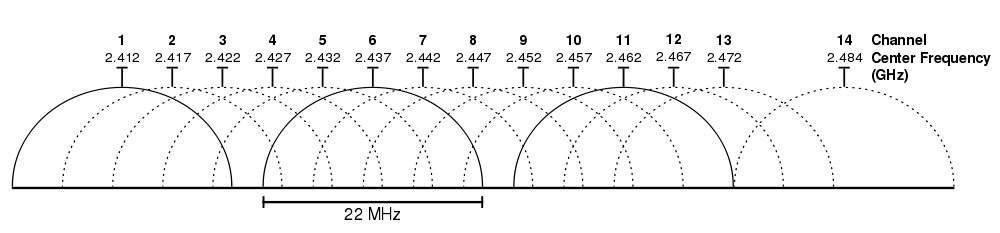
\includegraphics[width=1\textwidth]{wifichannels}
   \caption{Illustration of the Wi-Fi channels on the 2,4 GHz band. \cite{wifichannels}}
   \label{fig:wifichannels}
\end{figure}

Wi-Fi doesn't use frequency hopping to avoid data collisions. This forms a problem when there are hidden nodes in the network. A hidden node is illustrated in figure \ref{fig:hiddennode}. The circles indicate the transmission range of each node. In figure \ref{fig:hiddennode} 'A' is not in the transmission range of 'C', which makes 'A' invisible to 'C'. In this situation node A and C are not aware of eachother. Therefore one of the nodes can think that it is the only active node in the network.

\begin{figure}[H]
   \centering
   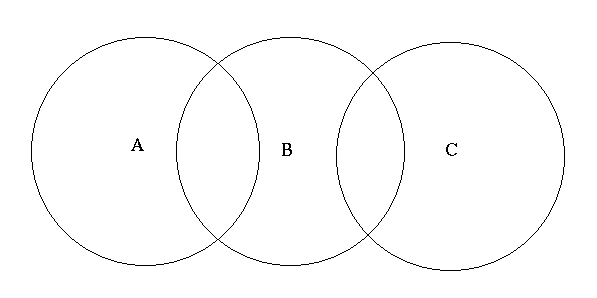
\includegraphics[width=1\textwidth]{hiddennodeproblem}
   \caption{Illustrates the hidden node problem with three nodes.}
   \label{fig:hiddennode}
\end{figure}

In the following situation there will be a collision of information:
\begin{itemize}
\setlength\itemsep{0em}
\item Node 'A' sends data to node 'B'.
\item Simultaniously node 'C' is also sending information to node 'B'.
\end{itemize}

Using handshake frames can be a solution to prevent a collision from happening when there is a hidden node. With 802.11, the used handshakes frames are CTS (clear to send) and RTS (request to send). The solution is given in figure \ref{fig:rtscts}. Where node 'A' send an RTS to 'B' and 'B' responds with an CTS to node 'A' and 'C'. Node 'C' didn't send an RTS, so the node knows that it needs to wait. The waiting duration of data transmission is contained in the CTS message which is send by node 'B'. \cite{tcipbook}

\begin{figure}[H]
   \centering
   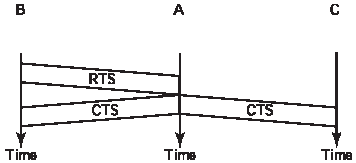
\includegraphics[width=.75\textwidth]{rtscts}
   \caption{Gives an example of the hidden node problem given in \ref{fig:hiddennode}}
   \label{fig:rtscts}
\end{figure}

As mentioned before, using handshake frames can be a solution to prevent a data collision from happening in case of a hidden node. However, in a exposed node problem, this method will cause data transmission inefficiency. \cite{tcipbook} Figure \ref{fig:exposedstation} illustrates the exposed node problem. In figure \ref{fig:rtscts2} the following situation is illustrated:

\begin{itemize}
\setlength\itemsep{0em}
\item Node 'A' wants to send information to the node 'B'.
\item Node 'C' also wants to send information to node 'D'.
\item Because node 'C' receives an RTS, it doesn't get permission to send an RTS itself.
\end{itemize}

\begin{figure}[H]
   \centering
   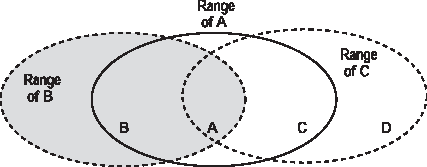
\includegraphics[width=1\textwidth]{exposedstation}
   \caption{The exposed node problem with four nodes and two nodes who want to send information.}
   \label{fig:exposedstation}
\end{figure}

\begin{figure}[H]
   \centering
   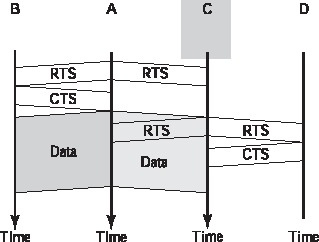
\includegraphics[width=.75\textwidth]{rtscts2}
   \caption{Gives an example of the exposed node problem given in \ref{fig:exposednode}}
   \label{fig:rtts2}
\end{figure}

\textbf{Summerization}\\
To summerize the given information from the protocols table \ref{sumtableprotocols} is made.

Network size
The networkssize of each of the protocols is expendable. A Bluetooth piconet for example can be part of a scatternet, which overlooks serveral other piconets. However, it is desireable that there are direct limitations in the network size




\textbf{Transmission time}\\
The transmission latency between nodes can be calculated with equation \ref{eq:transmissiontime}.\cite{comparitivestudywirelessprotocols} The data size ($N_{data}$), the maximum payload size ($N_{maxPld}$), the overhead size ($N_{ovhd}$), the bit time ($T_{bit}$) and the propagation time ($T_{prop}$) between devices form the transmission latency ($T_{tx}$). 

\begin{equation}
    T_{tx}=(N_{data} + \Bigg(\frac{N_{data}}{N_{maxPld}} N_{ovhd} \Bigg) T_{bit} + T_{prop})
    \label{eq:transmissiontime}
\end{equation}

When the data payload size increases the transmission time increases as shown in \cite{comparitivestudywirelessprotocols}. In comparison to the other protocols, UWB has the lowest bit time which results in the fastest tranmission time followed by Wi-Fi. Where ZigBee followed by Bluetooth have the slowest tranmission time.

\textbf{Protocol complexity}\\
The protocol complexity can be compared by the number of primitives and events in a set situation. When there are more primitives or events in a certain protocol, it indicates the complexity. \cite{comparitivestudywirelessprotocols} As indicated in figure \ref{fig:protocolcomplexity} Bluetooth is by far the most complex protocol compared to the other protocols.

\begin{figure}[H]
   \centering
   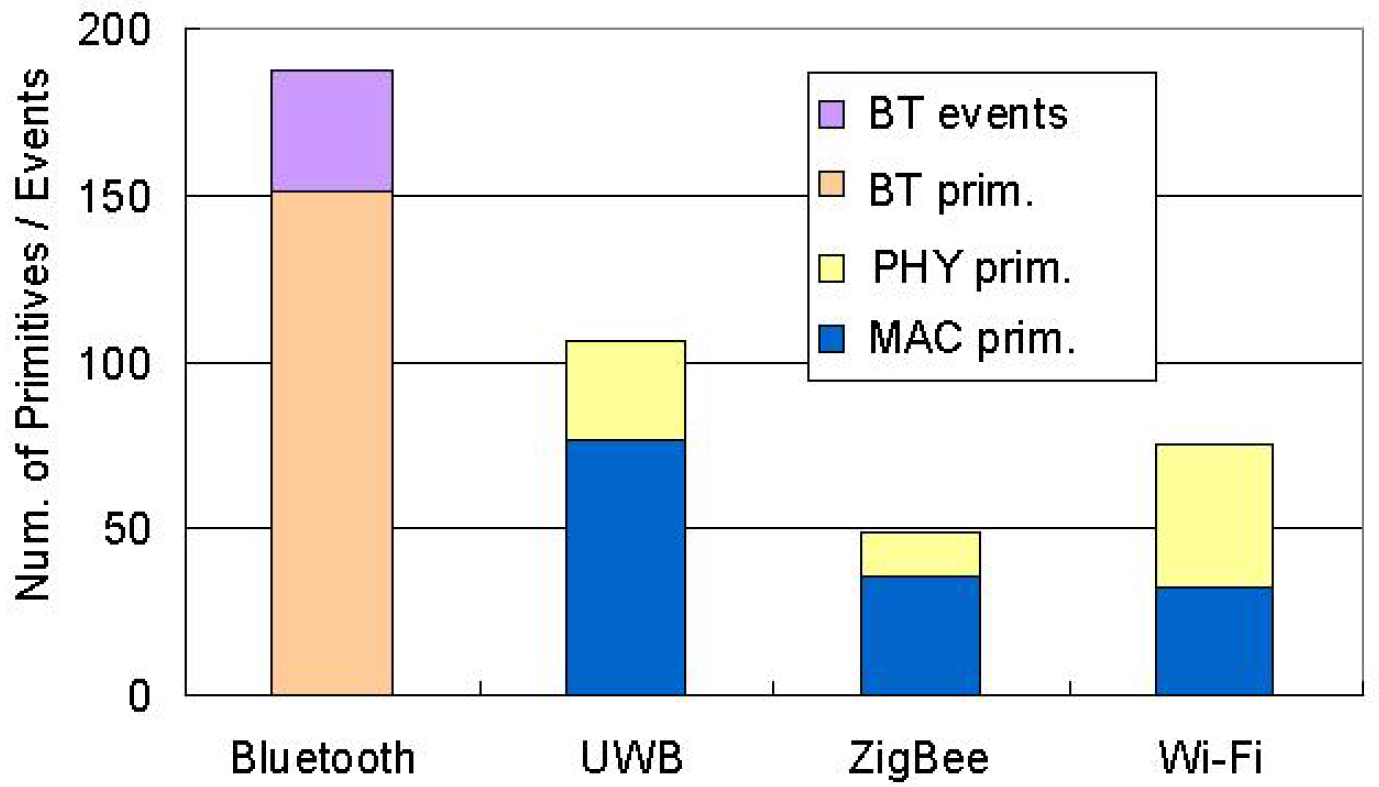
\includegraphics[width=1\textwidth]{protocolcomplexity}
   \caption{Comparision of the complexity for each protocol, found in \cite{comparitivestudywirelessprotocols}.}
   \label{fig:protocolcomplexity}
\end{figure}


Each of the discussed protocols has it's own complexity. The reasearch done in \cite{comparitivestudywirelessprotocols} compares them in data coding efficiency versus the data size. The data coding efficiency is based on the data and message size. The average ratio between the data and message size is the data coding efficiency percentage. 

\begin{figure}[H]
   \centering
   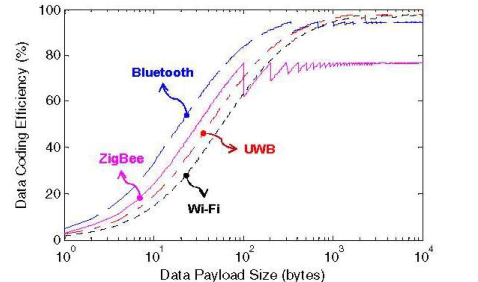
\includegraphics[width=1\textwidth]{datacodingefficieny}
   \caption{Comparision of the data coding efficiency for each protocol, found in \cite{comparitivestudywirelessprotocols}.}
   \label{fig:protocolefficiency}
\end{figure}

Figure \ref{fig:protocolefficiency} illustrates the data coding efficiency for each protocol. Bluetooth for example has the best data coding efficiency when using a small amount of bytes (around 339 bytes). Wi-FI and UWB on the otherhand are more efficient for large data sizes. Where Zigbee saturates on 80 percent efficiency when the data size increases.






\textbf{Power consumption}\\
The power consumption of each protocol depends on the used hardware. To make a valid comparison, the paper \cite{comparitivestudywirelessprotocols} made a selection of average hardware. The comparison in figure \ref{fig:protocolenergy} gives an indication of the average power consumption of each protocol. Bluetooth and ZigBee both consume about 100mW where the power consumption of UWB and Wi-Fi is about 700mW. Figure \ref{fig:protocolefficiency} gives the normalized energy consumption of each protocol. The normalized energy is given in mJ/Mb. The normalized energy consumption indicates that ZigBee and Bluetooth both use more energy to transceive the same amount of information. UWB is the most efficient protocol to transceive information.



\begin{figure}[H]
   \centering
   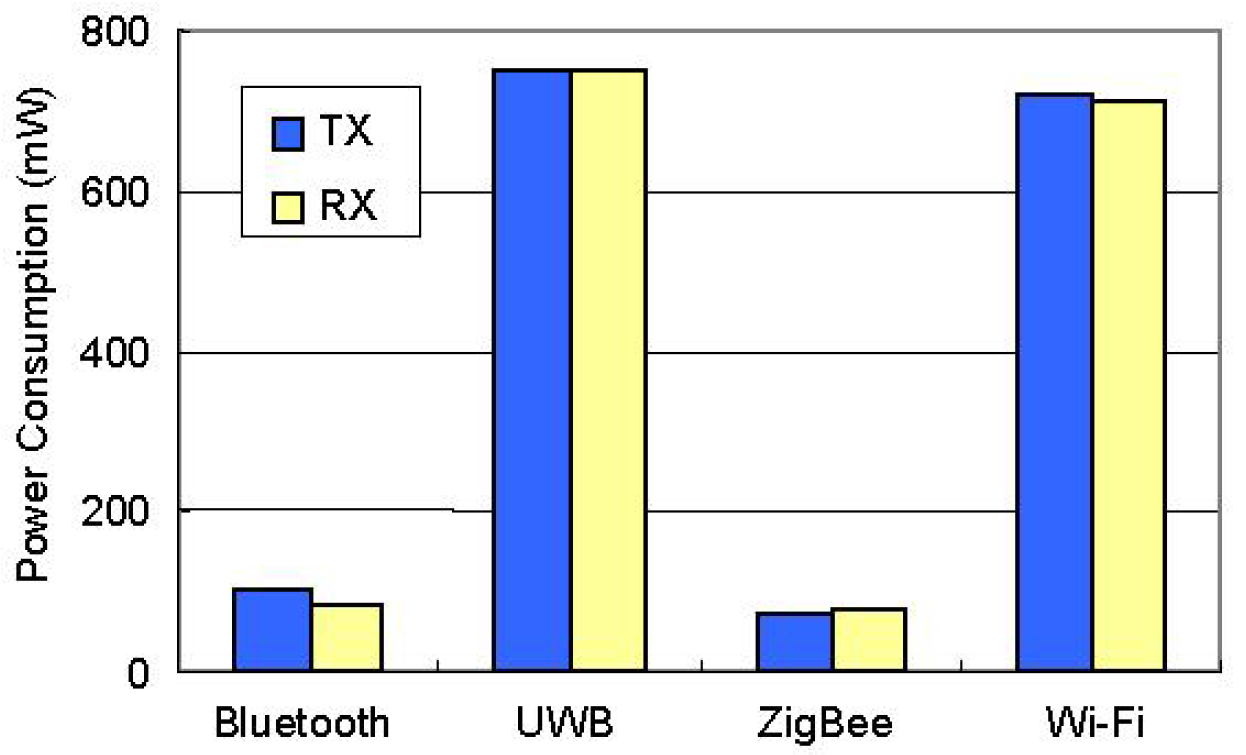
\includegraphics[width=1\textwidth]{images/protocolenergy.png}
   \caption{Comparision of the power consumption for each protocol, found in \cite{comparitivestudywirelessprotocols}.}
   \label{fig:protocolenergy}
\end{figure}

\begin{figure}[H]
   \centering
   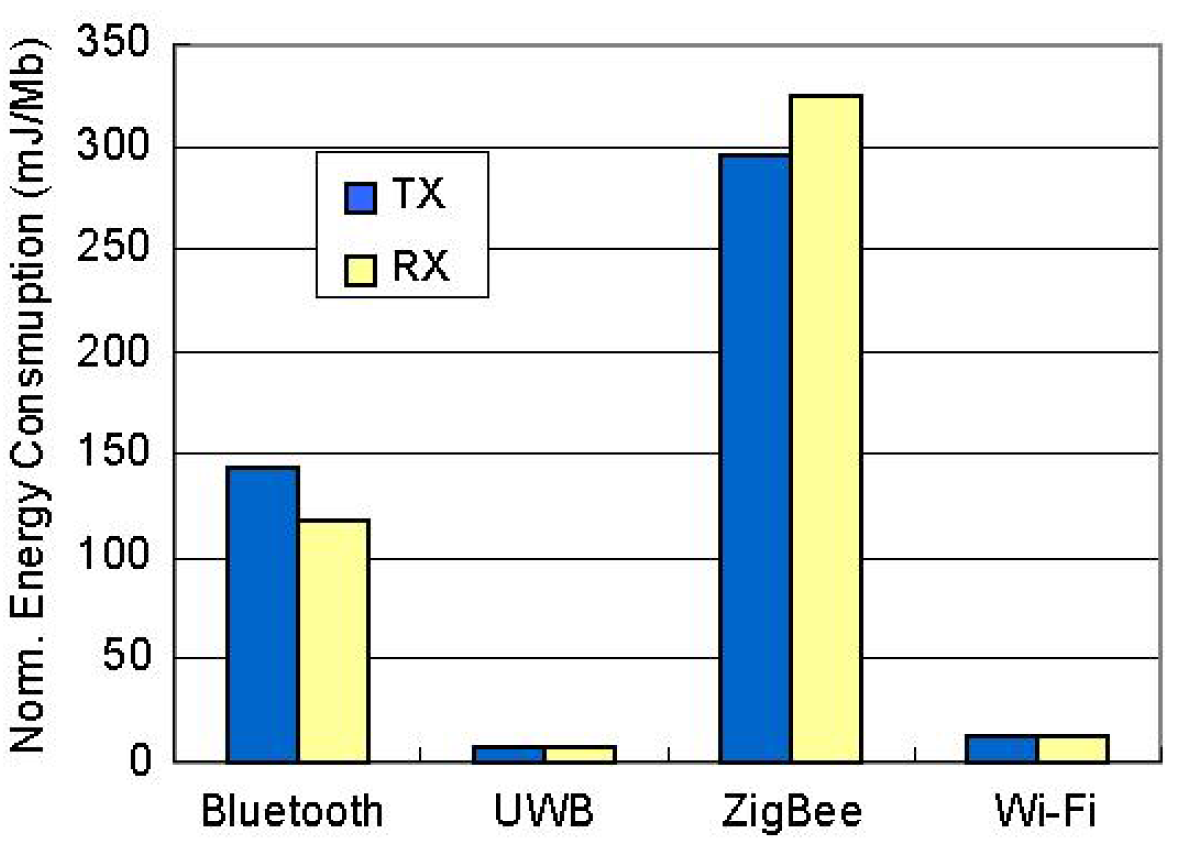
\includegraphics[width=1\textwidth]{images/protocolenergynormalized.png}
   \caption{Comparision of the normalized energy consumption for each protocol, found in \cite{comparitivestudywirelessprotocols}.}
   \label{fig:protocolenergynormalized}
\end{figure}


\begin{table}[H]
\centering
\caption{A table with a summirazing of the protocols. The table is based on information from \cite{comparitivestudywirelessprotocols}.}
\label{sumtableprotocols}
\resizebox{\textwidth}{!}{\begin{tabular}{|l|l|l|l|l|}
\hline
\textbf{Standard}        & \textbf{Bluetooth} & \textbf{Ultra-wide band} & \textbf{ZigBee}      & \textbf{Wi-Fi} \\ \hline
IEEE spec.               & 802.15.1           & 802.15.3a                & 802.15.4             & 802.11a/b/g    \\ \hline
Frequency band           & 2.4 GHz            & 3.1-10.6 GHz             & 868/915 MHz; 2,4 GHz & 2,4GHz; 5GHz   \\ \hline
Max signal rate          & 1Mb/s              & 110Mb/s                  & 250Kb/s              & 54Mb/s         \\ \hline
Nominal range            & 10m                & 10m                      & 10-100m              & 100m           \\ \hline
Channel bandwidth        & 1 MHz              & 500 MHz - 7.5 GHz        & 0.3/0.6 MHz; 2MHz    & 22 MHz         \\ \hline
Basic cell               & Piconet            & Piconet                  & Star                 & BSS            \\ \hline
Extension basic cell     & Scatternet         & Peer-to-peer             & Cluster tree, mesh   & ESS            \\ \hline
Max cell nodes & 8                  & 8                        & \textgreater65000    & 2007           \\ \hline
\end{tabular}}
\end{table}






\subsubsection{Conclusion}
In this section an substudy in swarm communication is made. The results of the substudy have resulted in recommendations for the implementation of the swarming module. An enumeration of the recommendations are given below:
\begin{itemize}
\setlength\itemsep{0em}
    \item The connection must be wireless due to the mobility of swarm members.
    \item Scaling on large-scale projects is not possible without using geographic locating (precize locating). \cite{geographicalrouting}\cite{scalablelocation}. 
    \item The network must be reliable, so it must use self-organization and topology control algorithms \cite{WMN1}
\end{itemize}

Nog onderzoeken:
Unicasting, multi-casting and broadcasting

Boek communicatie systemen blz:
827-834
845-849
450-453
438-443


\newpage



\subsection{Sensors}
For close range obstacle avoidance, the robots will need some kind of proximity sensing technique. The sensor needs to differentiate between different "treats" for the robot to function properly. For example; when the sensor detects a small hill, which the robot can move over it should not trigger the robot to move away from it. But when it detects a big obstacle it should trigger the robot to move away. This is important because the robots will eventually be expected to move across rough terrain (like Mars). In the next paragraphs some different proximity sensor techniques will be discussed. Price is also a important factor while comparing these techniques. Multiple robots must be made on a tight budget, so costs should be cut where possible.\\


\subsubsection{Ultrasoon sensor}
Een veel gebruikte proximity sensor op simpele robots is de ultrasoonsensor. Dit komt omdat deze in vergelijking tot andere sensoren een goedkope oplossing is. Een ultrasoon sensor stuurt een ultrasoon geluid uit dit geluid wordt teruggekaatst tegen het object en vervolgens weer opgevangen door de sensor. De tijd die het geluid er over gedaan heeft wordt gemeten. Met een simpel rekensommetje wordt vervolgens de afstand bepaald. Een probleem met de ultrasoon sensor is dat het moeilijk is om te discrimineren tussen verschillende objecten. Hierdoor wordt het moeilijk om onderscheid te maken tussen bijvoorbeeld een heuveltje (waar de robot wel overheen kan) en een obstakel die de robot moet ontwijken. Door de atmosfeer op mars wordt geluid ernstig gedempt hierdoor is ultrasoon niet implementeerbaar op mars \cite{soundonmars}. Voor testen op aarde is het echter wel een goed werkend en bewezen techniek.

\subsubsection{Lidar sensor}
Lidar staat voor “Light detection and ranging”. Deze sensor werkt volgens het zelfde principe als de ultrasoon sensor. Het is al bewezen dat de lidar techniek werkt op Mars. Met de Phoenix missie is er een lidar systeem gebruikt om wolken en atmosferische stof te meten\cite{lidarmars}. Het licht van de laser kon wolken meten op meerdere kilometers hoogte. Omdat licht zich zeer snel verplaatst, moet de elektronica in een lidar sensor ook snel zijn. Hierdoor is de prijs in vergelijking tot de ultrasoon sensor hoog.

\begin{figure}[!ht]

  \centering
      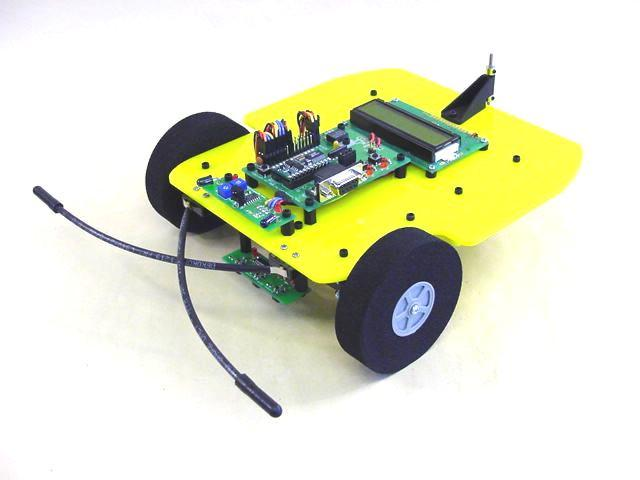
\includegraphics[width=0.5\textwidth]{voelsprieten.jpg}
  \caption{Robot met mechanische proximity sensor}  \label{voelspriet}
 
\end{figure}

\subsubsection{Mechanische sensor}
Eén mechanische proximity sensor bestaat meestal uit twee onderdelen. Dit zijn de actuator, dit is meestal een simpele druk schakelaar. En de arm of "bumper", dit is het deel dat het object aanstoot en zorgt dat de mechanishe kracht op de schakelaar wordt uitgeoefend figuur \ref{voelspriet} . De kracht van deze techniek is zijn eenvoudigheid. Er hoeven geen ingewikkelde signalen verwerkt te worden, enkel het aan of uit signaal van de actuator. Een groot nadeel van deze techniek is dat de sensor fysiek tegen een object aan moet komen om het te detecteren. In een zwerm van relatief fragiele robots is dit niet ideaal. Wanneer de robots zich op ruiger terrein bevinden, zal het gebruik van een "bumper" of arm ook niet ideaal zijn, deze kan namelijk vast blijven zitten tegen of achter obstakels.



\subsubsection{Sensor choice for the robot}
Now the question is which of the different sensor techniques proposed, is the best to implement on the swarm robots. While answering this question the following points will be taken into account:

\begin{itemize}
    \item The sensor must be easy to reproduce because multiple robots must be made from the swarm.
    \item The budget is limited, therefore the sensor price should be cheap compared the the total price of one robot.
    \item Energy usage should be as low as possible to increase the operation time per robot.
    \item For budget reasons there has been chosen to not take into account if the sensor would work on Mars.
\end{itemize}

Looking at these points it becomes clear that the lidar sensor wouldn't be the best choice. It doesn't really have any outstanding pros compared to the other two techniques and it's much more expensive. Currently the cheapest lidar sensor would cost about 100$\euro$. The ultrasonic and mechanical sensor wouldn't cost more than a few Euro's. As talked about before the mechanical sensor has a few drawbacks compared to the ultrasonic sensor. For these reasons the ultrasonic sensor seems the best choice. The only issue left to solve is how to sense the difference between obstacles which the robot has to avoid, and things the robot doesn't have to avoid, but still might be detected by the sensor. This will be discussed in the next paragraph.

\subsubsection{Obstacle discrimination with an ultrasonic sensor}
An ultrasonic sensor is usually used to detect if there is some obstacle in the way. In this case there is made no difference made between a obstacle that the robot can move over, or a obstacle that should be avoided. For example: a small slope or hill might be detected as an obstacle, but in truth the robot can move over it. The robots developed for this program will eventually be able to cross harsh terrain. In this case the proximity sensor will need to discriminate between these situations. Working with ultrasonic waves there are multiple domains to work with. These are time, frequency and amplitude. Time is used to determine the distance between the object and the sensor. The change in frequency and/or amplitude contains information about the shape of the object\cite{ultraobject}. 
In the paper "Object recognition with ultrasonic sensor" is concluded 
that looking at the amplitude over time contains enough information to discriminate between object\cite{ultraobject}. The example is given of an object with separated surfaces of 3,5cm, the echo from the second surface will be delayed by 0,2msec relative to the echo from the first surface. This delay can be easily detected with a microprocessor. The reason looking at frequency isn't the first choice is because of the higher hardware requirements it would require to properly sample the signal. 
\\

\newpage

\section{Bibliography}
\bibliography{references}
\bibliographystyle{IEEEtran}



\end{document}